\section{Temporal stability}
The following section will be looking at the results from choosing different $\theta$ values in our scheme. The benchmark test FSI-2 has been used to with a pretty high time step $ k = 0.01$. We only study the effects of lift as the three other quantities shows the same behavior.   
\begin{figure}[H]
\label{fig:lift_shifted}
\caption{LiftShifted}
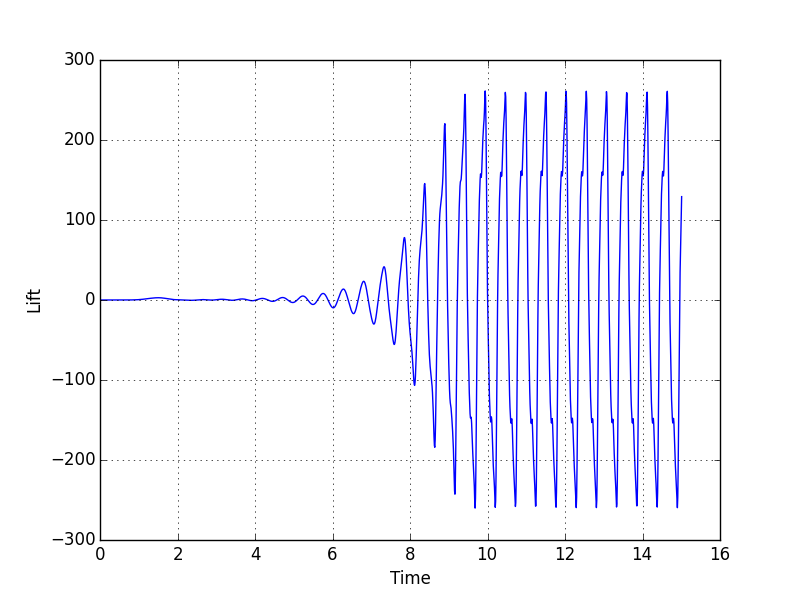
\includegraphics[scale=0.6, trim={0mm 0mm 0mm 0mm},clip]{./Verification_Validation/Temporal_stability/lift_shifted.png}
\end{figure}
